\documentclass[a4paper,12pt]{report}

\usepackage{alltt, fancyvrb, url}
\usepackage{graphicx}
\usepackage[utf8]{inputenc}
\usepackage{float}
\usepackage{xcolor}
\usepackage{hyperref}
\usepackage[inkscapelatex=false]{svg}

\usepackage[italian]{babel}

\usepackage[italian]{cleveref}

\title{
RisiKOOP \\
\begin{large}
Il gioco strategico per la conquista del mondo
\end{large}
}

\author{Matteo Caruso, Matteo Ceccarelli, Franceso Sacripante}
\date{\today}


\begin{document}

\maketitle

\tableofcontents

\chapter{Analisi}

\section{Descrizione e requisiti}

Il software mira a replicare il gioco Risiko, un gioco da tavolo di strategia a turni dove ogni giocatore controlla una squadra di unità allo scopo di completare un obiettivo determinato da una Carta Obiettivo pescata a inizio partita.
Questa richiederà di conquistare dei continenti, annientare un'altra armata oppure conquistare un certo numero di territori.
Il gioco inizia spartendo tutti i territori tra i giocatori e dà dei territori iniziali con cui rinforzarli.
Ogni turno turno, il giocatore otterrà vari carri armati da posizionare sui suoi territori.
Potrà poi attaccare territori adiacenti ai propri.
Se riesce a conquistare almeno uno stato otterrà una Carta Territorio, utilizzabile per giocare combo al fine di ottenere ulteriori unità nei successivi turni.
Infine avrà l'opportunità di spostare delle unità fra i suoi territori.

\subsubsection{Tipi di Combo}
Le combo sono sempre tris di carte territorio, ognuna ricompensa un certo numero di unità:
\begin{itemize}
	\item 3 cannoni: 4 unità.
	\item 3 fanti: 6 unità.
	\item 3 cavalieri: 8 unità.
	\item Un fante, un cannone e un cavaliere: 10 unità. \footnote{Non è possibile sostituire una delle carte con un Jolly in questa combo.}
	\item Un Jolly e due carte uguali: 12 unità.
\end{itemize}

\subsubsection{Requisiti funzionali}
\begin{itemize}
	\item Il software dovrà permettere di giocare a una semplice versione di Risiko.
	\item Ogni giocatore ha una sua Carta Obiettivo e varie Carte Territorio.
	\item L'attacco avviene tramite il tiro di dadi, il cui confronto ne determinerà l'esito.
\end{itemize}

\subsubsection{Requisiti non funzionali}
\begin{itemize}
	\item La mappa è selezionabile, scelta dai giocatori a inizio partita.
	\item I giocatori dovranno poter nascondere le proprie Carte Obiettivo e Territorio agli altri giocatori.
\end{itemize}

\section{Modello del Dominio}

Il gioco inizia con la selezione dei giocatori, del loro colore e della mappa.
Successivamente vengono assegnati i territori, ed è chiesto ai giocatori di posizionare le loro unità rimanenti in quei territori.
Ora inizia il game-loop del gioco, che si ripete fino a quando un giocatore non vince:
\begin{itemize}
	\item Fase di rinforzo.
	\item Fase di attacco.
	\item Fase di spostamento strategico.
\end{itemize}

\begin{figure}[H]
	\centering
	\includesvg[width=1\textwidth]{svg/analysis-model.svg}
	\caption{UML del modello svolto dopo l'analisi dei requisiti.}
\end{figure}

\chapter{Design}

\section{Architetura}

L'architettura del software è basata su un pattern Model-View-Controller (MVC).
L'entry point dell'applicazione è il \texttt{Controller}, che si occupa di avviare il model, che implementa \texttt{GameManager}, e le view registrate, che implementano \texttt{RisikoView}.
La separazione permette di aggiungere facilmente altre \texttt{RisikoView} se necessario, senza compromettere la logica del model e del controller.

Le fasi di gioco sono state modellate con una \begin{itshape}State Machine\end{itshape}, un paradigma di programmazione che permette di dividere il sistema in varie sotto-fasi, detti anche \begin{itshape}stati\end{itshape}. Ogni fase ha la prporia logica diversa da quella di tutte le altre. Nel programma si risconoscono perché implementano \texttt{GamePhase}.
Questo paradigma favorisce il \begin{itshape}Single Responsibility Principle\end{itshape}, siccome ogni fase è responabile internamente della propria gestione.
Un'altro vantaggio risiede nella chiarezza con qui descrive in che punto dell'esecuzione si trova l'applicazione, siccome può essere in una sola fase.
% TODO: UML delle interfacce per tutti i controller, il game manager e la risiko view.

\section{Design dettagliato}
\subsection{Matteo Caruso}
\subsubsection{Validare le combo di carte}
\paragraph{Problema}
Bisogna validare vari tipi di combo di carte, ognuna con requisiti diversi. Inoltre ogni combo ricompensa il giocatore con un numero di unità diverso.
\paragraph{Soluzione}
\begin{figure}[H]
	\centering
	\includesvg[width=1\textwidth]{svg/detailed_design-combo_check_strategy.svg}
	\caption{UML del pattern Strategy per la validazione delle combo.}
\end{figure}
La validazione delle combo usa il pattern \begin{itshape}Strategy\end{itshape}, in cui ogni validatore di combo è una strategia diversa.
\\
Il pattern \begin{itshape}Strategy\end{itshape} è più adatto rispetto al pattern \begin{itshape}Template Method\end{itshape}, siccome ogni validatore di combo differisce molto dagli altri, fatta eccezione dei validatori \texttt{AllEqualCombo}.

\subsubsection{Validare le \texttt{AllEqualCombo}}
\paragraph{Problema}
Bisogna validare le combo di carte dove hanno tutte lo stesso tipo.
\paragraph{Soluzione}
\begin{figure}[H]
	\centering
	\includesvg[width=1\textwidth]{svg/detailed_design-all_equal_combo_template_method.svg}
	\caption{UML del pattern Template Method per la validazione delle combo di carte con tipo uguale.}
\end{figure}
Qui è possibile usare il pattern \begin{itshape}Template Method\end{itshape}, dove la classe astratta \texttt{AllEqualCombo} definisce il template method \texttt{comboIsValid} e l'operazione primitiva \texttt{getUnitType} \footnote{Restituisce \texttt{UnitType}, un enumeratore che rappresenta i semi delle carte.}.
\\
Gli lascia anche la responsabilità di implementare \texttt{getUnitRewardAmount}. Le classi che estendono questa classe astratta sono \texttt{AllCannonEqualCombo}, \texttt{AllJackEqualCombo} e \texttt{AllKnightEqualCombo}, che implementano l'operazione primitiva sopracitata.

\subsection{Matteo Ceccarelli}
\subsubsection{Gestione del mazzo di carte obiettivo}
\paragraph{Problema}
Non essendo la mappa fissa, è necessario realizzare delle carte obbiettivo che si adattassero dinamicamente alla configurazione della mappa selezioanta.
\paragraph{Soluzione}
Ho usato il pattern \textit{Template method}.
Creo una classe astratta \texttt{AbstractObjectiveCardBuilder} che incorpora la logica di creazione delle carte espondo i metodo astratti primitivi \texttt{buildDescription} e \texttt{buildSpecification}, che genera la carta mediante il metodo template \texttt{createCard}. Ho preferito l'utilizzo del \textit{template method} rispetto al \textit{pattern startegi} perchè mi permetteva meglio di isolare nelle classi che ereditano la \texttt{AbstractObjectiveCardBuilder} unicamente gli elementi che differiscono tra i le varie tipologie, incorparando gli aspetti comuni legati alla loro creazione.

\subsubsection{Composizione delle condizioni di vittoria con Specification Pattern}
\paragraph{Problema}
Avere un modo semplice, espressiovo e componibile per definire e controllare la condizzione di vittoria delle carte obbiettivo, che spesso condividono aspetti di logiche comuni, come ad esempio conquinsta X territorio, o conquista almeno N territori con almeno M truppe.
\paragraph{Soluzione}
Lo specification pattern mi permette di rispondere a questa esegenza e, mediante la combinazione logica di tante piccole condizioni atomiche, mi consente di realizzare espressioni logiche più o meno complesse. La parte centrale del pattern risiede nell'interfaccia funzionale \texttt{Specification} che espone i metodi \texttt{and}, \texttt{or}, \texttt{not} repsonsabile della composizione delle varie specifiche.
%```java
%@FunctionalInterface
%public interface Specification<T> {
%    boolean isSatisfiedBy(T candidate);
%
%    default Specification<T> and(Specification<T> other) { … }
%    default Specification<T> or(Specification<T> other) { … }
%    default Specification<T> not() { … }
%}
%```
%
I vantaggi introdotti da questo pattern mi hanno portato a preferire questa soluzione, all' alternative di Strategy che non si presatava al riutilizzo di logiche comuni, come ad esempio conquista N territori.
La scelta dello Specification Pattern si è rivelata dunque la più adatta per astrarre la logica di verifica dell'obiettivo dalla costruzione della carta, massimizzando il riuso e mantenendo il design pulito e modulare.

\subsubsection{Gestione delle fasi di gioco}
\paragraph{Problema}
RisikOOP è un gioco a turni in cui, in base alla fase corrente, gli stessi eventi della GUI (ad es. \texttt{selectTerritory} o \texttt{performAction}) devono produrre comportamenti diversi.
\paragraph{Soluzione}
Si è adottato il pattern \textit{Strategy}, modellando ogni fase di gioco come una strategia indipendente, aderente all'interfaccia base \texttt{GamePhase}.
%```java
%   public interface GamePhase {
%     boolean selectTerritory(Territory t);
%     boolean isComplete();
%   }
%```
In Più dato che non tutti gli eventi interessano ogni fase del gioco si è scelto di creare tante piccole interfacce ogniuna responsabile di incapsulare la logica di un'azione specifica, così facendo ogni fase implentava unicamnete le interfacce delle azzioni corrispondenti.
\subsection{Francesco Sacripante}
\subsubsection{Creazione della logica delle prime due fasi}
\paragraph{Problema}
Le prime due fasi hanno due logiche diverse tra loro e tra il resto del gioco
\paragraph{Soluzione}
Scomporre il controller in diversi dipi di controller.
\begin{figure}[H]
	\centering
	\includesvg[width=1\textwidth]{svg/detailed-design-multiple-cont-sacripante.svg}
	\caption{UML dei vari controller per le prime due fasi di gioco.}
\end{figure}
Risiko è un software molto legato alla visualizzazione del gioco, quindi per favorire il \begin{itshape}Separation of Concerns\end{itshape}, il controller è diviso in sotto-controller: \texttt{DataAddingContrller} permette di impostare giocatori e la mappa, mentre \texttt{DataRetrieveController} favorisce l'ottenimento di informazioni quali il giocatore corrente. Infine \texttt{TurnManager} permette di gestire le fasi del gioco.
\subsubsection{Aggiornamento dei colori dei territori della view}
\paragraph{Problema}
Durante il gioco, se un giocatore conquista un territorio, questo deve istantaneamente cambiare colore nel colore del nuovo proprietario.
\paragraph{Soluzione}
\begin{figure}[H]
	\centering
	\includesvg[width=1\textwidth]{svg/Observer-view-Sacripante.svg}
	\caption{UML del observer pattern usato per aggiornare gli elementi delle view.}
\end{figure}
Usare un'interfaccia dedicata agli aggiornamenti della view.
\\
Ogni volta che al model succede una cosa, il controller chiama i metodi dell'interfaccia per aggiornare la view.
Il patter usato quì è una sorta di observer pattern, dove l'observer è la view che viene "notificata" quando un territorio cambia proprietà e il soggetto è il territorio.
\subsubsection{Accorpamento di detentori di oggetti}
\paragraph{Problema}
Alcuni oggetti condividono la detenzione ed alcuni tipi di operazioni su alcuni tipi di oggetti posseduti.
Ci sono ogetti che detengono più territori o più giocatori.
\paragraph{Soluzione}
\begin{figure}[H]
	\centering
	\includesvg[width=1\textwidth]{svg/detailed-design-holders-sacripante.svg}
	\caption{UML degli holders del gioco.}
\end{figure}
Si creano delle interfaccie in cui si accorpano tutte le operazione in comune riguardante un certo insieme di oggetti.
% TODO: Design individuale da fare.


\chapter{Sviluppo}

\section{Testing automatizzato}
Il testing automatizzato è stato realizzato tramite JUnit, focalizzato principalmente sul model, come l'insermineto della mappa, la gestione dei giocatori, la validazione delle combo di carte, e sulla gestione delle fasi di gioco.
L'interfaccia grafica è stata testata manualmente durante lo sviluppo del software.

\section{Note di sviluppo}
% TODO: Note di sviluppo individuale da fare con permalink a github su feature di linguaggio di cui vai fiero.

\chapter{Commenti finali}

\section{Autovalutazione e lavori futuri}
% Obbligatorio individuale.

\section{Difficoltà incontrate e commenti per i docenti}
% Opzionale individuale.

\appendix
\chapter{Guida utente}
\section{Avviare la partita}
Prima di iniziare la partita bisogna definire i giocatori e la mappa su cui giocare.
\subsection{Inserire i giocatori}
\begin{figure}[H]
	\centering
	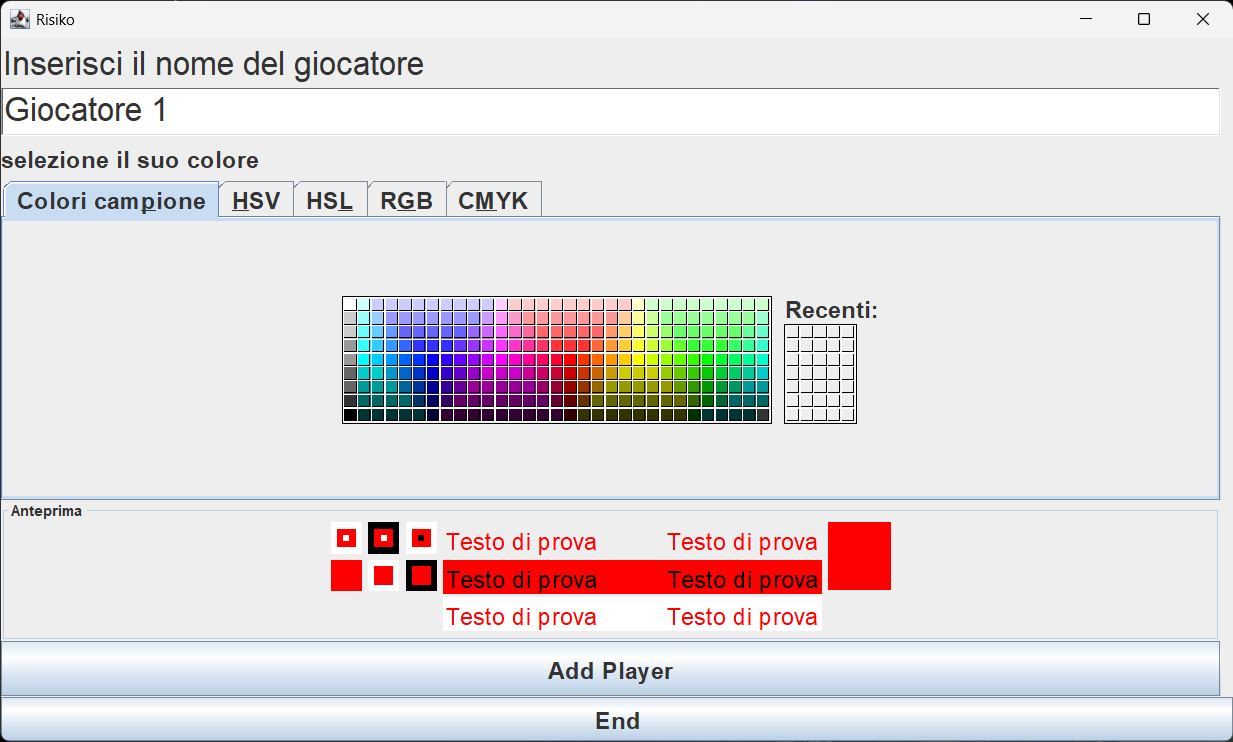
\includegraphics[width=1\textwidth]{user_guide/1_add_player.png}
	\caption{Schermata di aggiunta giocatori.}
\end{figure}
Per inserire un giocatore, scrivere il suo nome e selezionare il suo colore. Infine cliccare sul pulsante \textbf{Add Player}.
Ripetere il procedimento per ogni giocatore (almeno due), ricordando che sia il nome che il colore devono essere univoci.

Per concludere la scelta del giocatore, premere il pulsante \textbf{End}.
\subsection{Scegliere la mappa}
\begin{figure}[H]
	\centering
	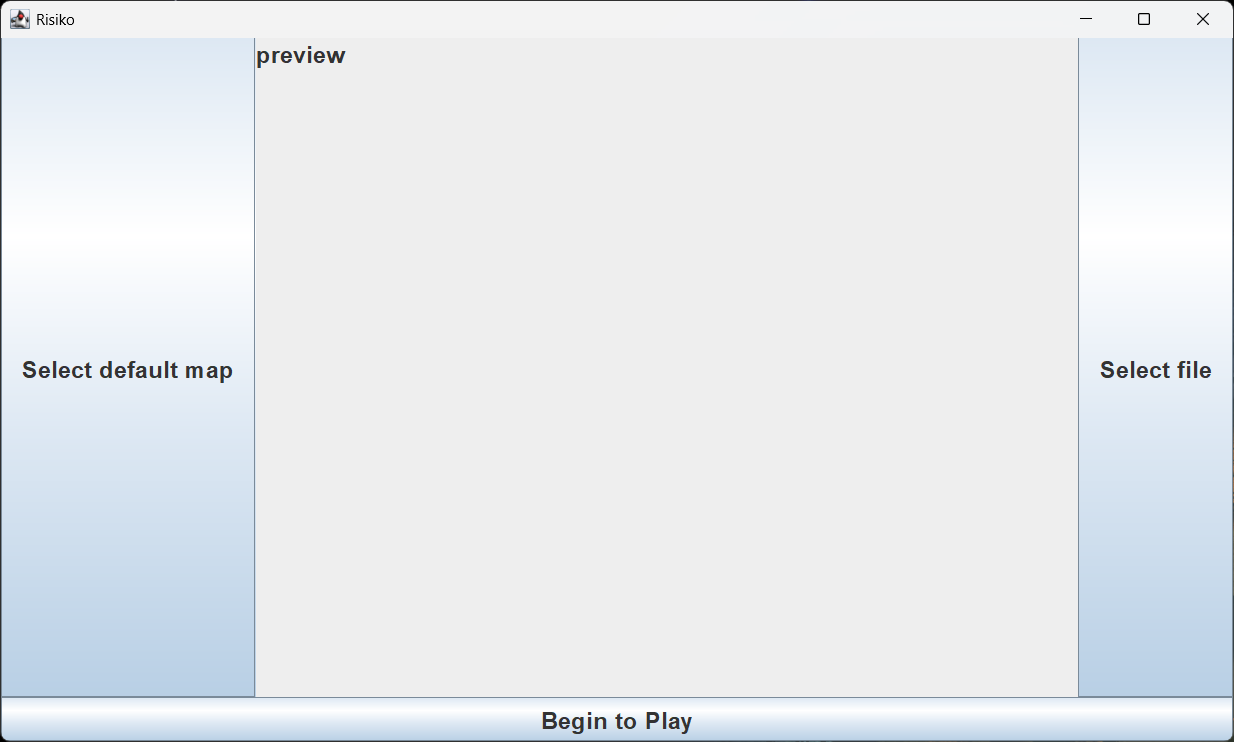
\includegraphics[width=1\textwidth]{user_guide/2_select_map_before.png}
	\caption{Schermata di selezione mappa.}
\end{figure}
Cliccare il pulsante \textbf{Select default map} per usare la mappa di default, altrimenti cliccare su \textbf{Select file} per scegliere un file \texttt{json} contenente i dati della mappa.
In caso di successo, verrà visualizzata l'anteprima della mappa selezionata.
\begin{figure}[H]
	\centering
	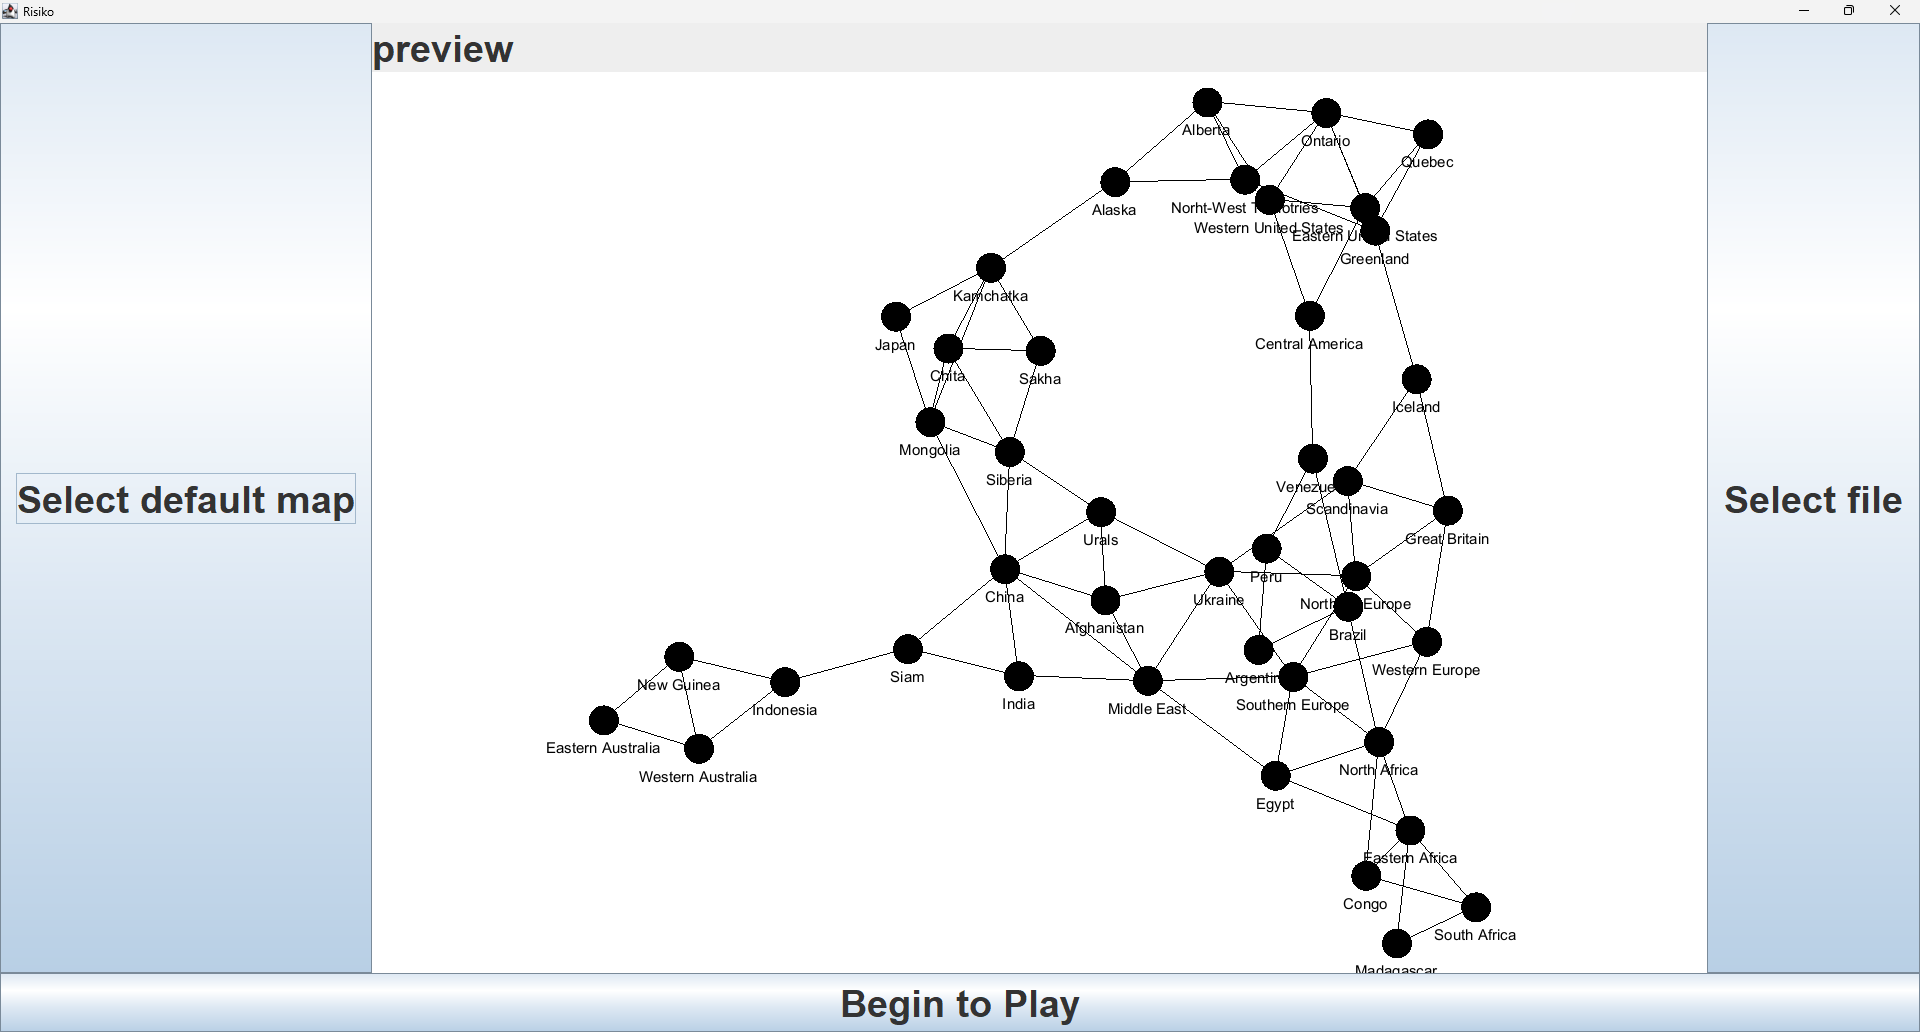
\includegraphics[width=1\textwidth]{user_guide/3_select_map_after.png}
	\caption{Anteprima della mappa selezionata.}
\end{figure}
Una volta completata la scelta, cliccare sul pulsante \textbf{Begin to Play} per iniziare la partita.

\section{Rinforzi iniziali}
\begin{figure}[H]
	\centering
	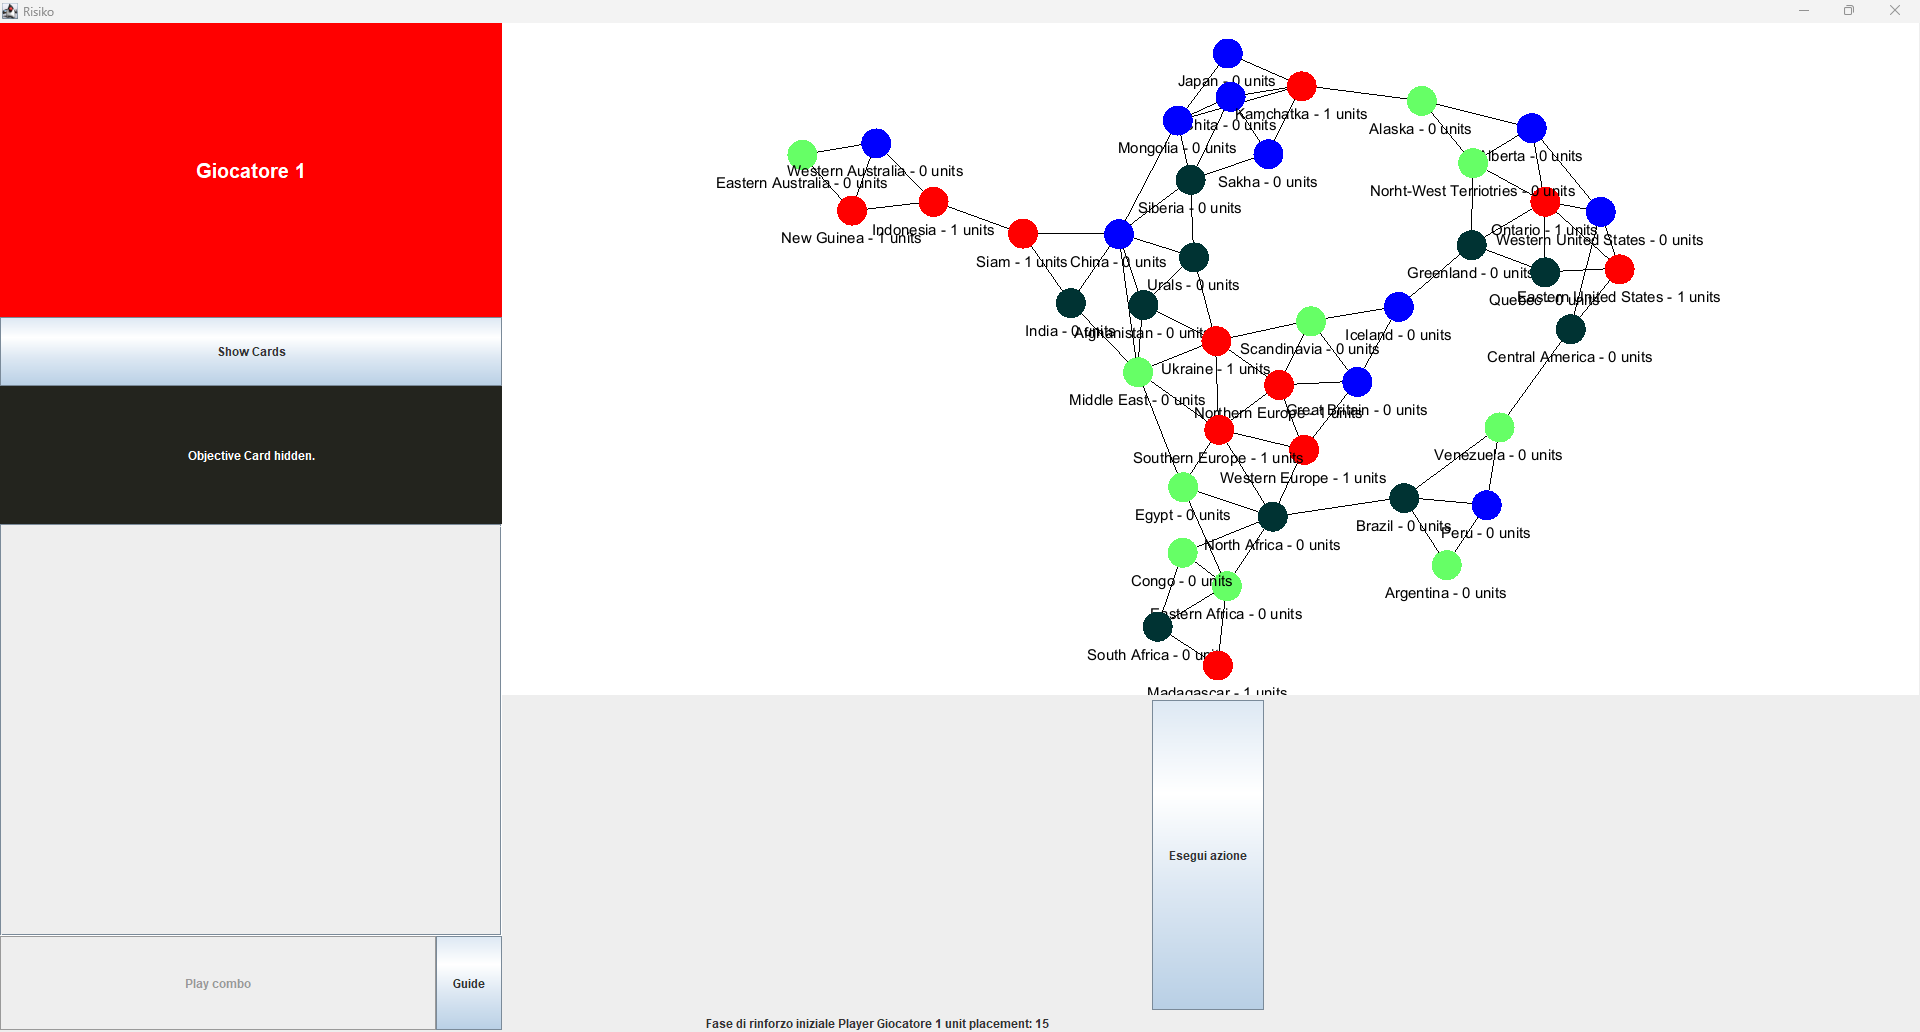
\includegraphics[width=1\textwidth]{user_guide/4_initial_reinforcements.png}
	\caption{Schermata di gioco iniziale.}
\end{figure}
I territori sono assegnati randomicamente ad ogni giocatore e viene posizionata un'unità su ogni territorio.
Ora a turno i giocatori posizionano le unità a loro rimaste. Il contatore è mostrato nel pannello inferiore. Cliccare su un territorio in possesso a quel giocatore per rinforzarlo fino a quando sono state posizionate tutte le unità. Infine cliccare sul pulsante \textbf{Esegui azione} per permettere al giocatore successivo di rinforzare i propri territori.

\subsubsection{Spostare e selezionare i nodi del grafo}
È possibile trascinare i nodi del grafo per spostare i nodi in caso si sovrappongano.
Se non è possibile spostare o cliccare i nodi del grafo, impostare il ridimensionamento dello schermo a 100\%. È un bug noto con la libreria Graphstream che stiamo utilizzando.
\begin{itemize}
	\item Stackoverflow: \url{https://
		      stackoverflow.com/questions/74860061/graphstream-2-0-mouse-pointer-offset-when-dragging-nodes-not-solved}
	\item Github: \url{https://github.com/graphstream/gs-core/issues/301}
\end{itemize}
\section{Schermata di gioco}
La fase di preparazione è stata completata. D'ora in avanti si svolgerà il turno di gioco normale fino alla vittoria di un giocatore.
La mappa è mostrata in alto a destra, dove il colore del territorio rappresenta il giocatore che lo possiede.
Il pannello a sinistra mostra informazioni relative al giocatore corrente.
È possibile visualizzare o nascondere la visibilità di dati privati, ovvero le carte e l'obiettivo, cliccando sul pulsante \textbf{Show Cards}.
\begin{figure}[H]
	\centering
	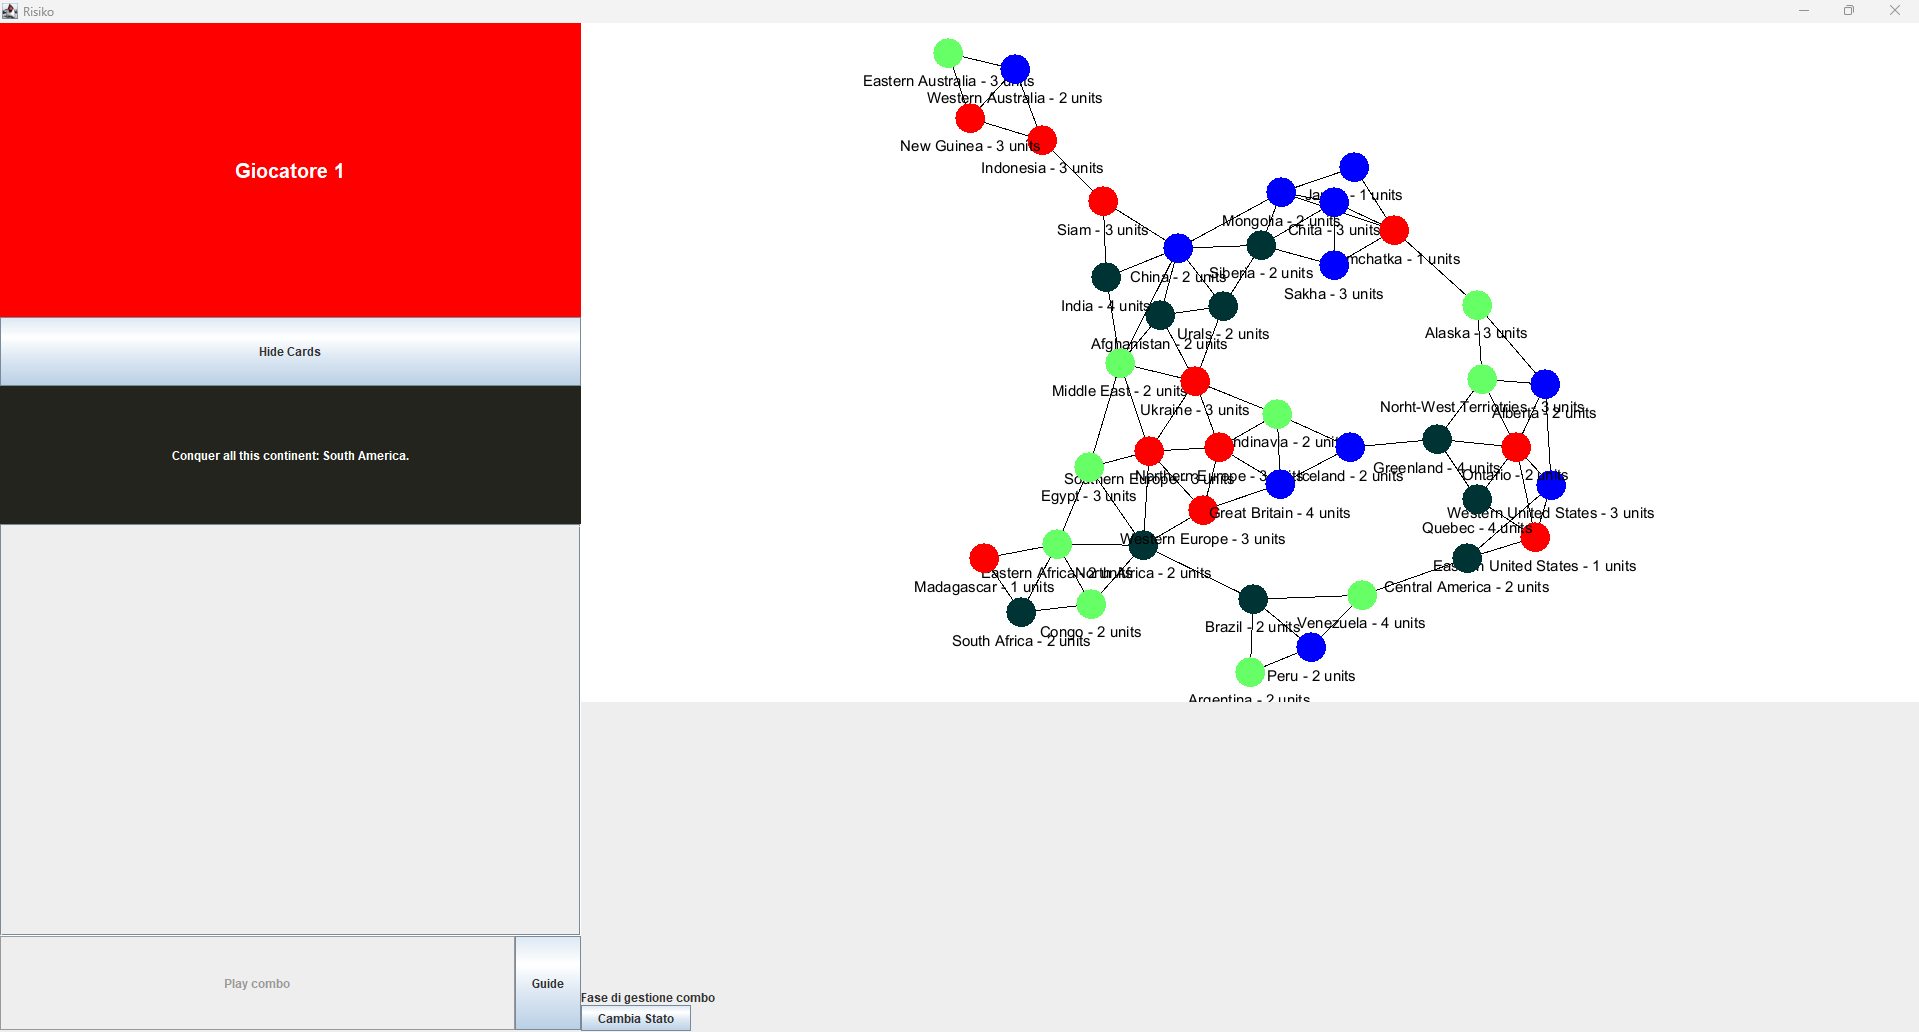
\includegraphics[width=1\textwidth]{user_guide/5_game_screen_show.png}
	\caption{Schermata di gioco con carte visibili.}
\end{figure}
È possibile visualizzare la lista di continenti e territori cliccando sul pulsante \textbf{Guide}.
\begin{figure}[H]
	\centering
	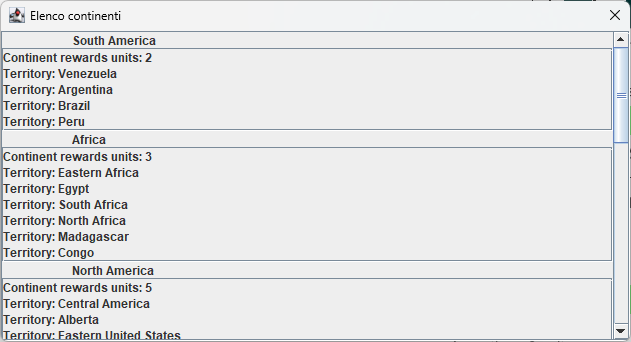
\includegraphics[width=1\textwidth]{user_guide/6_continent_list.png}
	\caption{Guida ai continenti e territori.}
\end{figure}
\subsection{Tipi di obiettivi}
\begin{itemize}
	\item Sconfiggere un determinato giocatore o conquistare 24 territori.
	\item Conquistare 18 territori e occuparli tutti con almeno 2 unità.
\end{itemize}



% TODO: Write list of objective cards

\section{Fase dei rinforzi}
La fase di rinforzi permette di rinforzare i territori all'inizio di ogni turno.
Il giocatore ottiene tante unità quanti sono i territori da lui occupati diviso tre, arrotondato per difetto.
Inoltre, se il giocatore possiede tutti i territori di un continente, ottiene un bonus specifico per quel continente, visibile nella Guida.
\subsection{Giocare le combo}
\begin{figure}[H]
	\centering
	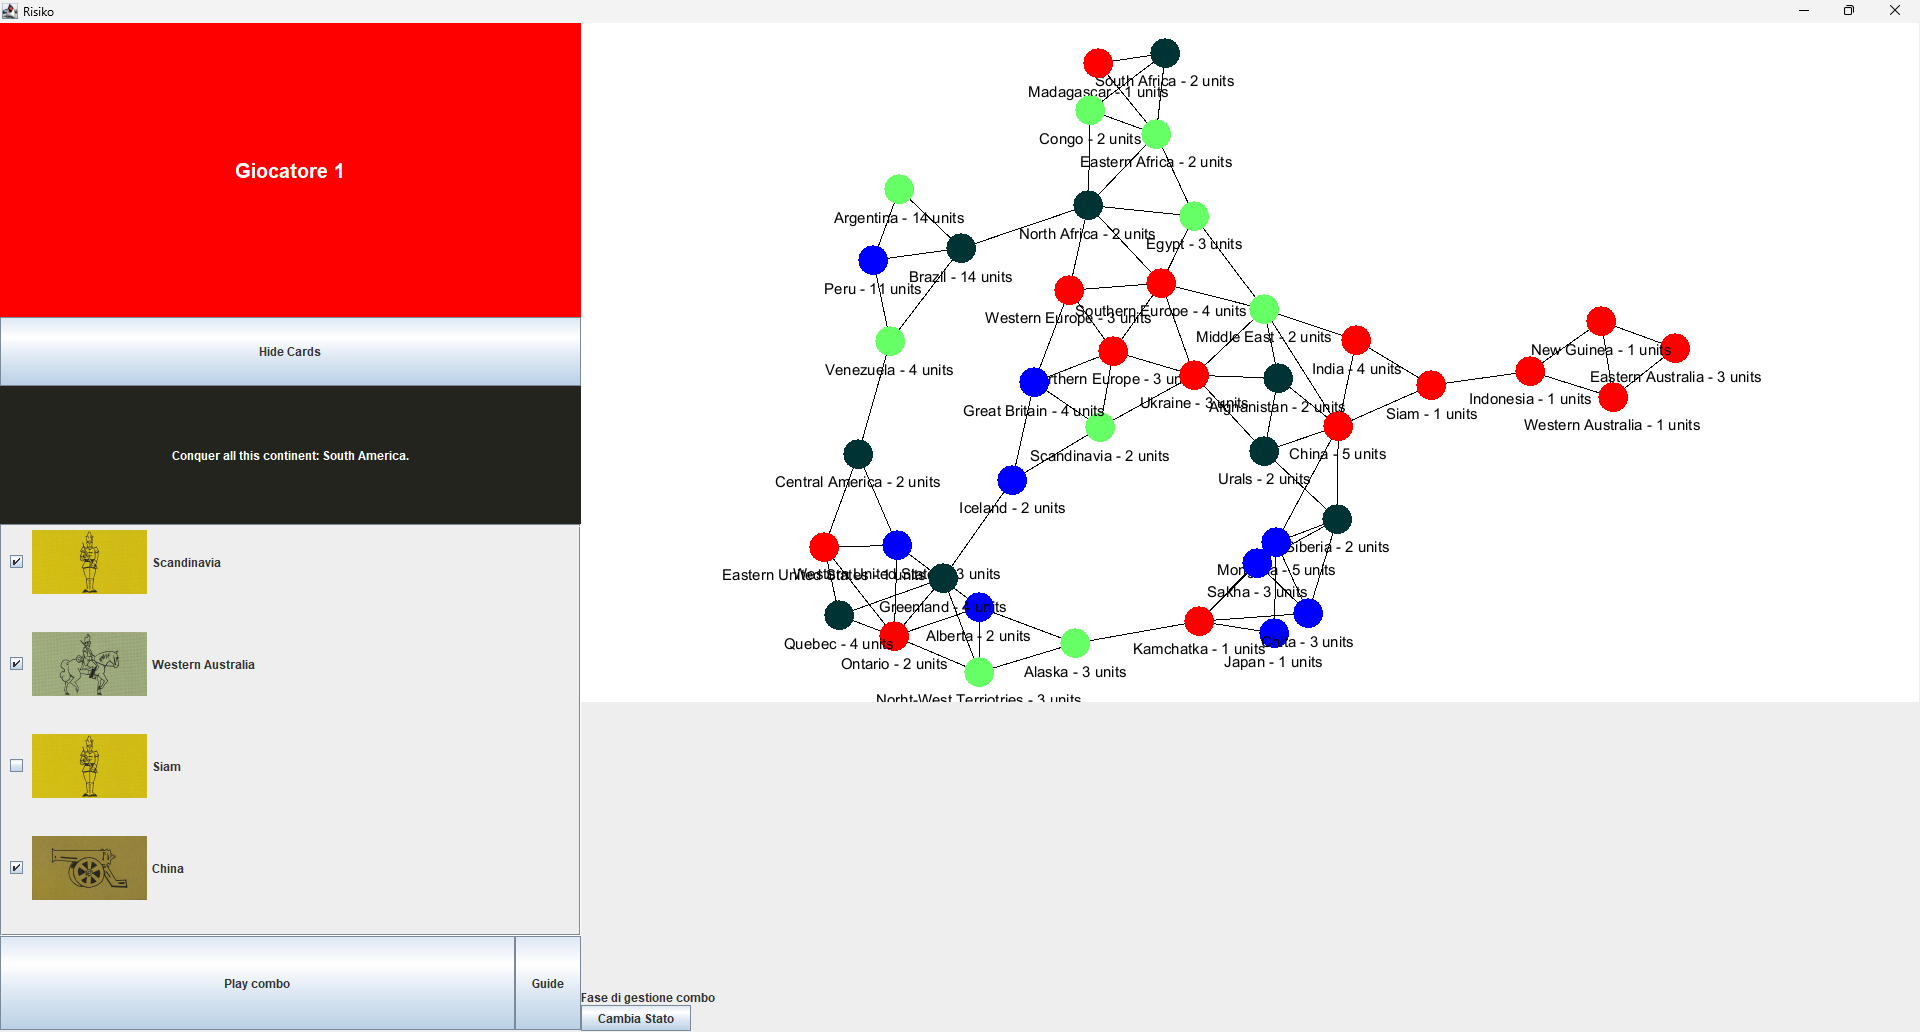
\includegraphics[width=1\textwidth]{user_guide/7_playing_combo.png}
	\caption{Carte valide selezionate per giocare una combo.}
\end{figure}

Prima di posizionare le unità, il giocatore può giocare una o più combo di carte. Per ottenere una carta, un giocatore deve conquistare almeno un territorio durante la fase di attacco del suo turno.
Ogni carta ha un seme (\textbf{Canone}, \textbf{Fante}, \textbf{Cavaliere}) e un territorio.
Nel mazzo sono presenti anche due carte \textbf{Jolly}.
\\
Le combo utilizzabili sono le seguenti:
\begin{itemize}
	\item 3 cannoni: 4 unità.
	\item 3 fanti: 6 unità.
	\item 3 cavalieri: 8 unità.
	\item Un fante, un cannone e un cavaliere: 10 unità.
	\item Un Jolly e due carte uguali: 12 unità.
\end{itemize}
Per giocare una combo, selezionare le \textit{checkbox} delle carte da giocare e cliccare sul pulsante \textbf{Play Combo}, che si attiverà solo se la combo è valida.

Sia che il giocatore abbia giocato una combo o meno, cliccare sul pulsante \textbf{Cambia stato} per passare alla fase di posizionamento delle unità.
\subsection{Aggiungere unità}
\begin{figure}[H]
	\centering
	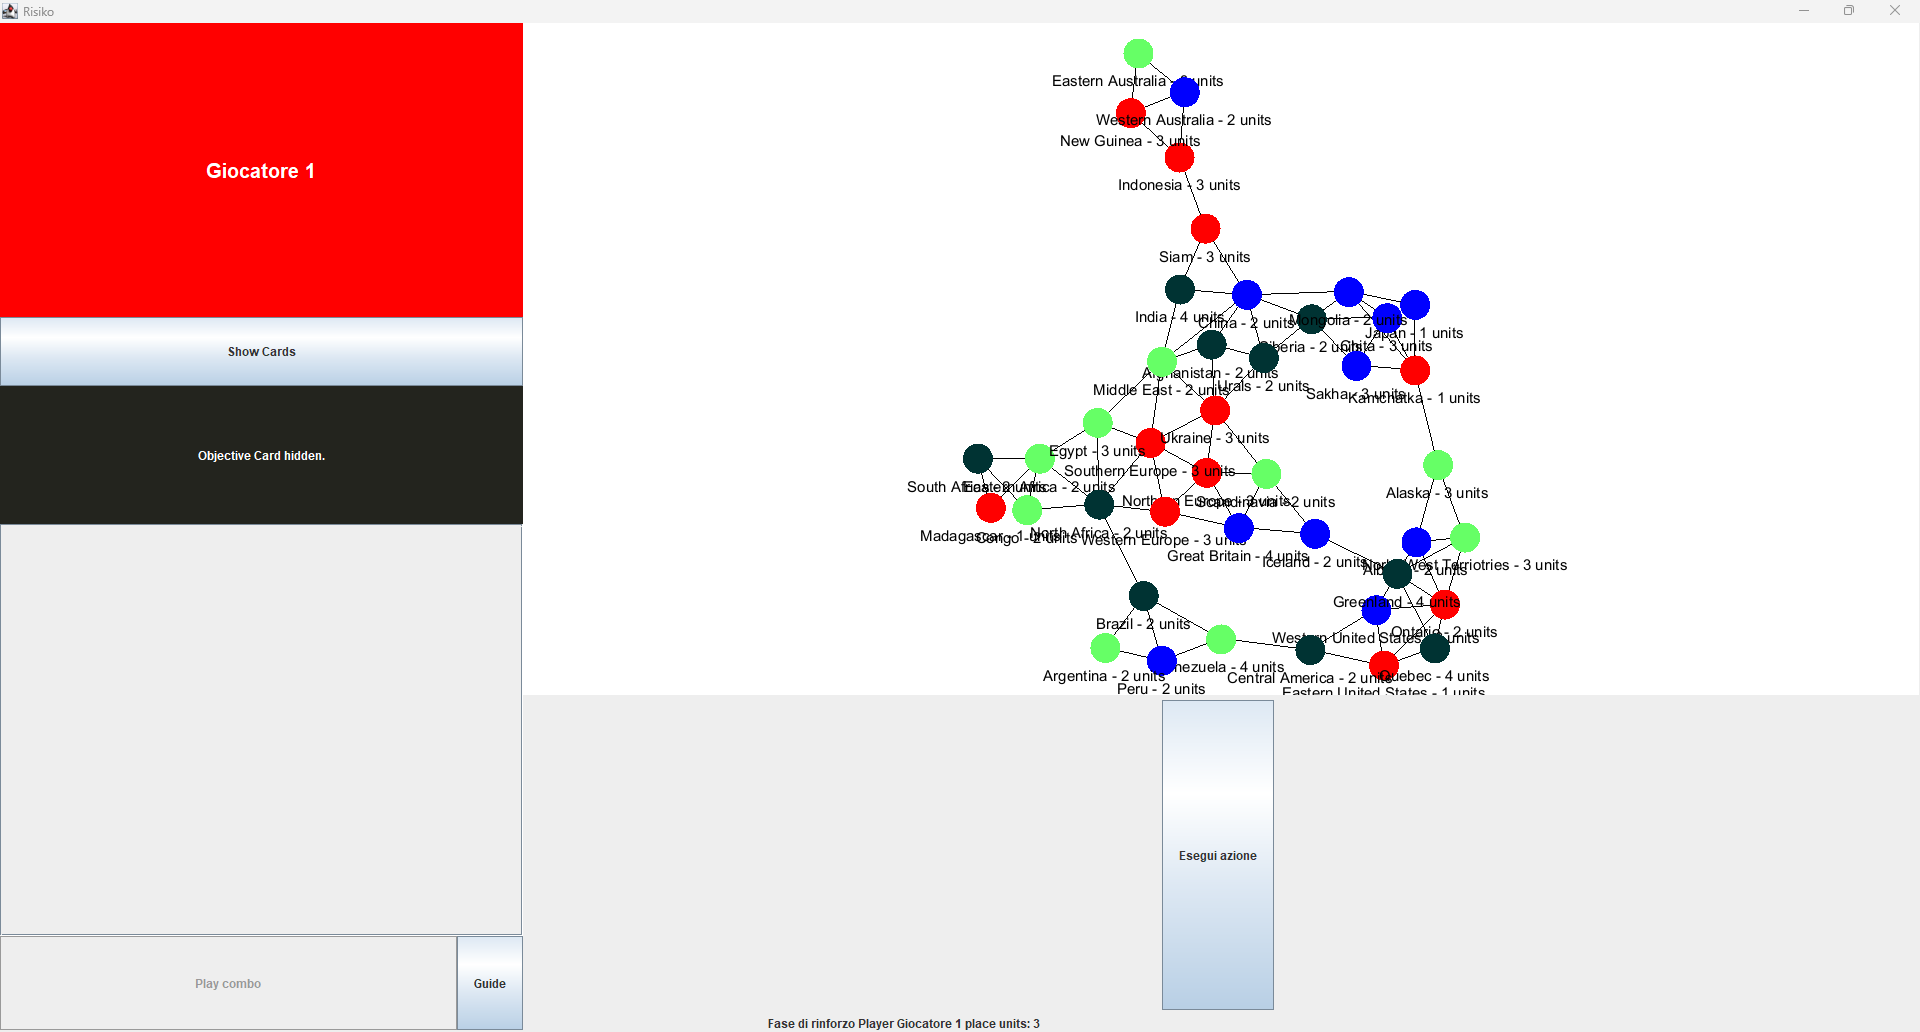
\includegraphics[width=1\textwidth]{user_guide/8_reinforcements.png}
	\caption{Fase di rinforzo.}
\end{figure}
L'aggiunta di unità sui territori del giocatore avviene come nella fase di rinforzi iniziali, ovvero cliccando sui territori nella mappa fino ad averle posizionate tutte.
Una volta posizionate tutte le unità, cliccare sul pulsante \textbf{Esegui azione} per passare alla fase di attacco.

\section{Fase di attacco}
La fase di attacco permette a un giocatore di utilizzare le unità posizionate su un suo territorio per attaccare e conquistare un territorio adiacente di un altro giocatore.

Occorre pianificare l'attacco in vari passaggi, dopo ognuno bisonga cliccare il pulsante \textbf{Esegui azione} per passare al passaggio successivo:
\begin{enumerate}
	\item Cliccare il territorio con cui attaccare, facendo attenzione che abbia un territorio nemico adiacente e che sia occupato da almeno due unità.
	\item Cliccare il territorio da attaccare. Dev'essere adiacente al territorio con cui si sta attaccando.
	\item Scegliere con quante untià bisogna svolgere l'attacco. Un massimo di 3 untià possono essere usate per attaccare, ma in caso di conquista del territorio tutte le unità definite qui saranno spostate nel territorio conquistato. Il numero di unità con cui attaccare deve essere compreso tra uno e il numero di unità del territorio con cui si sta attaccando meno uno.
\end{enumerate}

\begin{figure}[H]
	\centering
	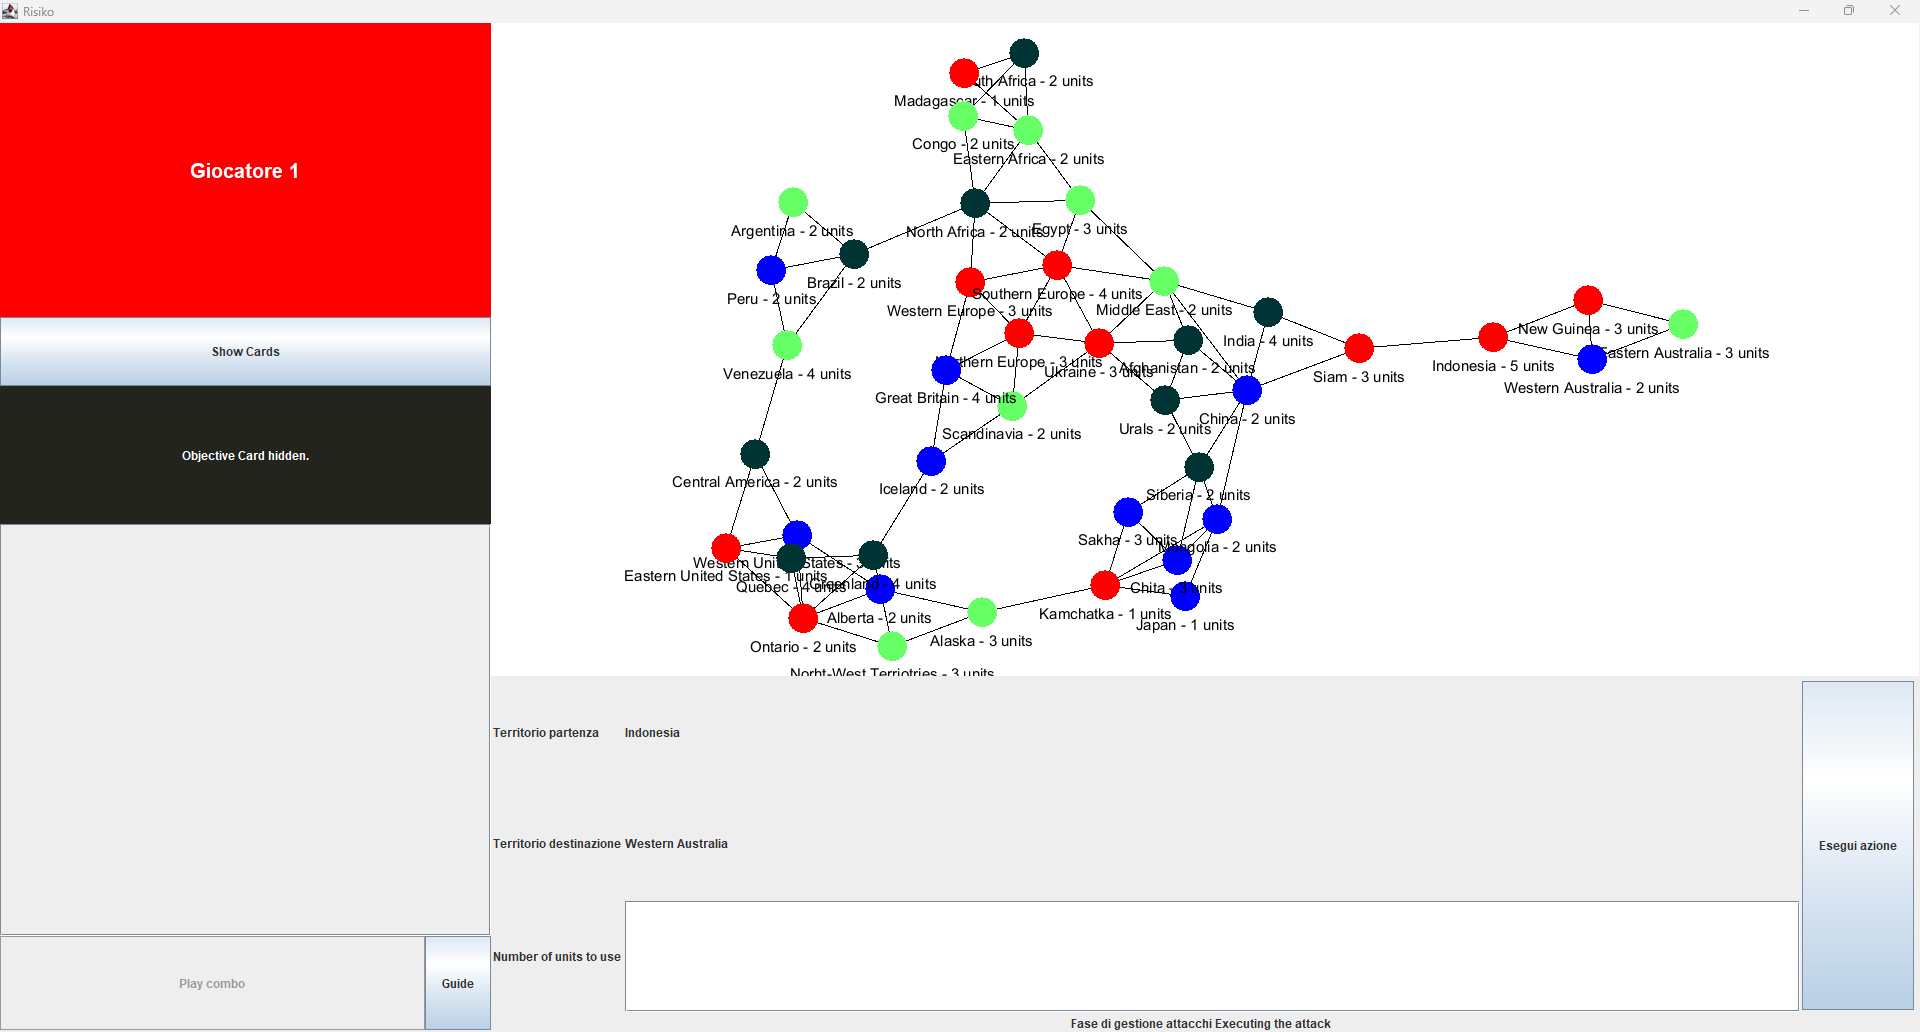
\includegraphics[width=1\textwidth]{user_guide/9_excecuting attack.png}
	\caption{Fase di attacco tra Indonesia e Australia Occidentale.}
\end{figure}

Per eseguire l'attacco tirando i dadi bisogna cliccare sul pulsante \textbf{Esegui azione}.
A seconda dell'esito dell'attacco, le unità perdenti saranno rimosse dai territori.
Nel caso in cui le unità difensori sconfitte siano state le ultime unità presenti su quel territorio, esso sarà conquistato dal giocatore attaccante, e tutte le unità attaccanti rimaste saranno spostate nel territorio conquistato.


Se durante la fase di attacco il giocatore ha conquistato almeno un territorio, otterrà una Carta Territorio, che sarà utilizzabile per giocare combo nei turni successivi.
Il giocatore corrente potrà decidere di effettuare altri attacchi o passare alla fase di spostamento strategico cliccando sul pulsante \textbf{Cambia stato}.

\subsubsection{Tiro di dadi}
\begin{figure}[H]
	\centering
	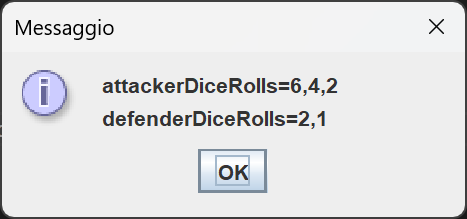
\includegraphics[width=0.5\textwidth]{user_guide/10_dice_rolls.png}
	\caption{Tiro di dadi.}
\end{figure}

L'attacco avviene tramite il tiro di dadi.
Vengono tirati tanti dadi quante le unità attaccanti (massimo 3) e tanti dadi quante le unità difensori (massimo 3).
I risultati dei dadi vengono ordinati in ordine decrescente e confrontati tra loro.
Per ogni coppia di risultati, il dado attaccante deve essere strettamente maggiore di quello difensore per sconfiggere un'unità difensore, in caso contrario sarà un'unità attaccante a perdere.
\begin{figure}[H]
	\centering
	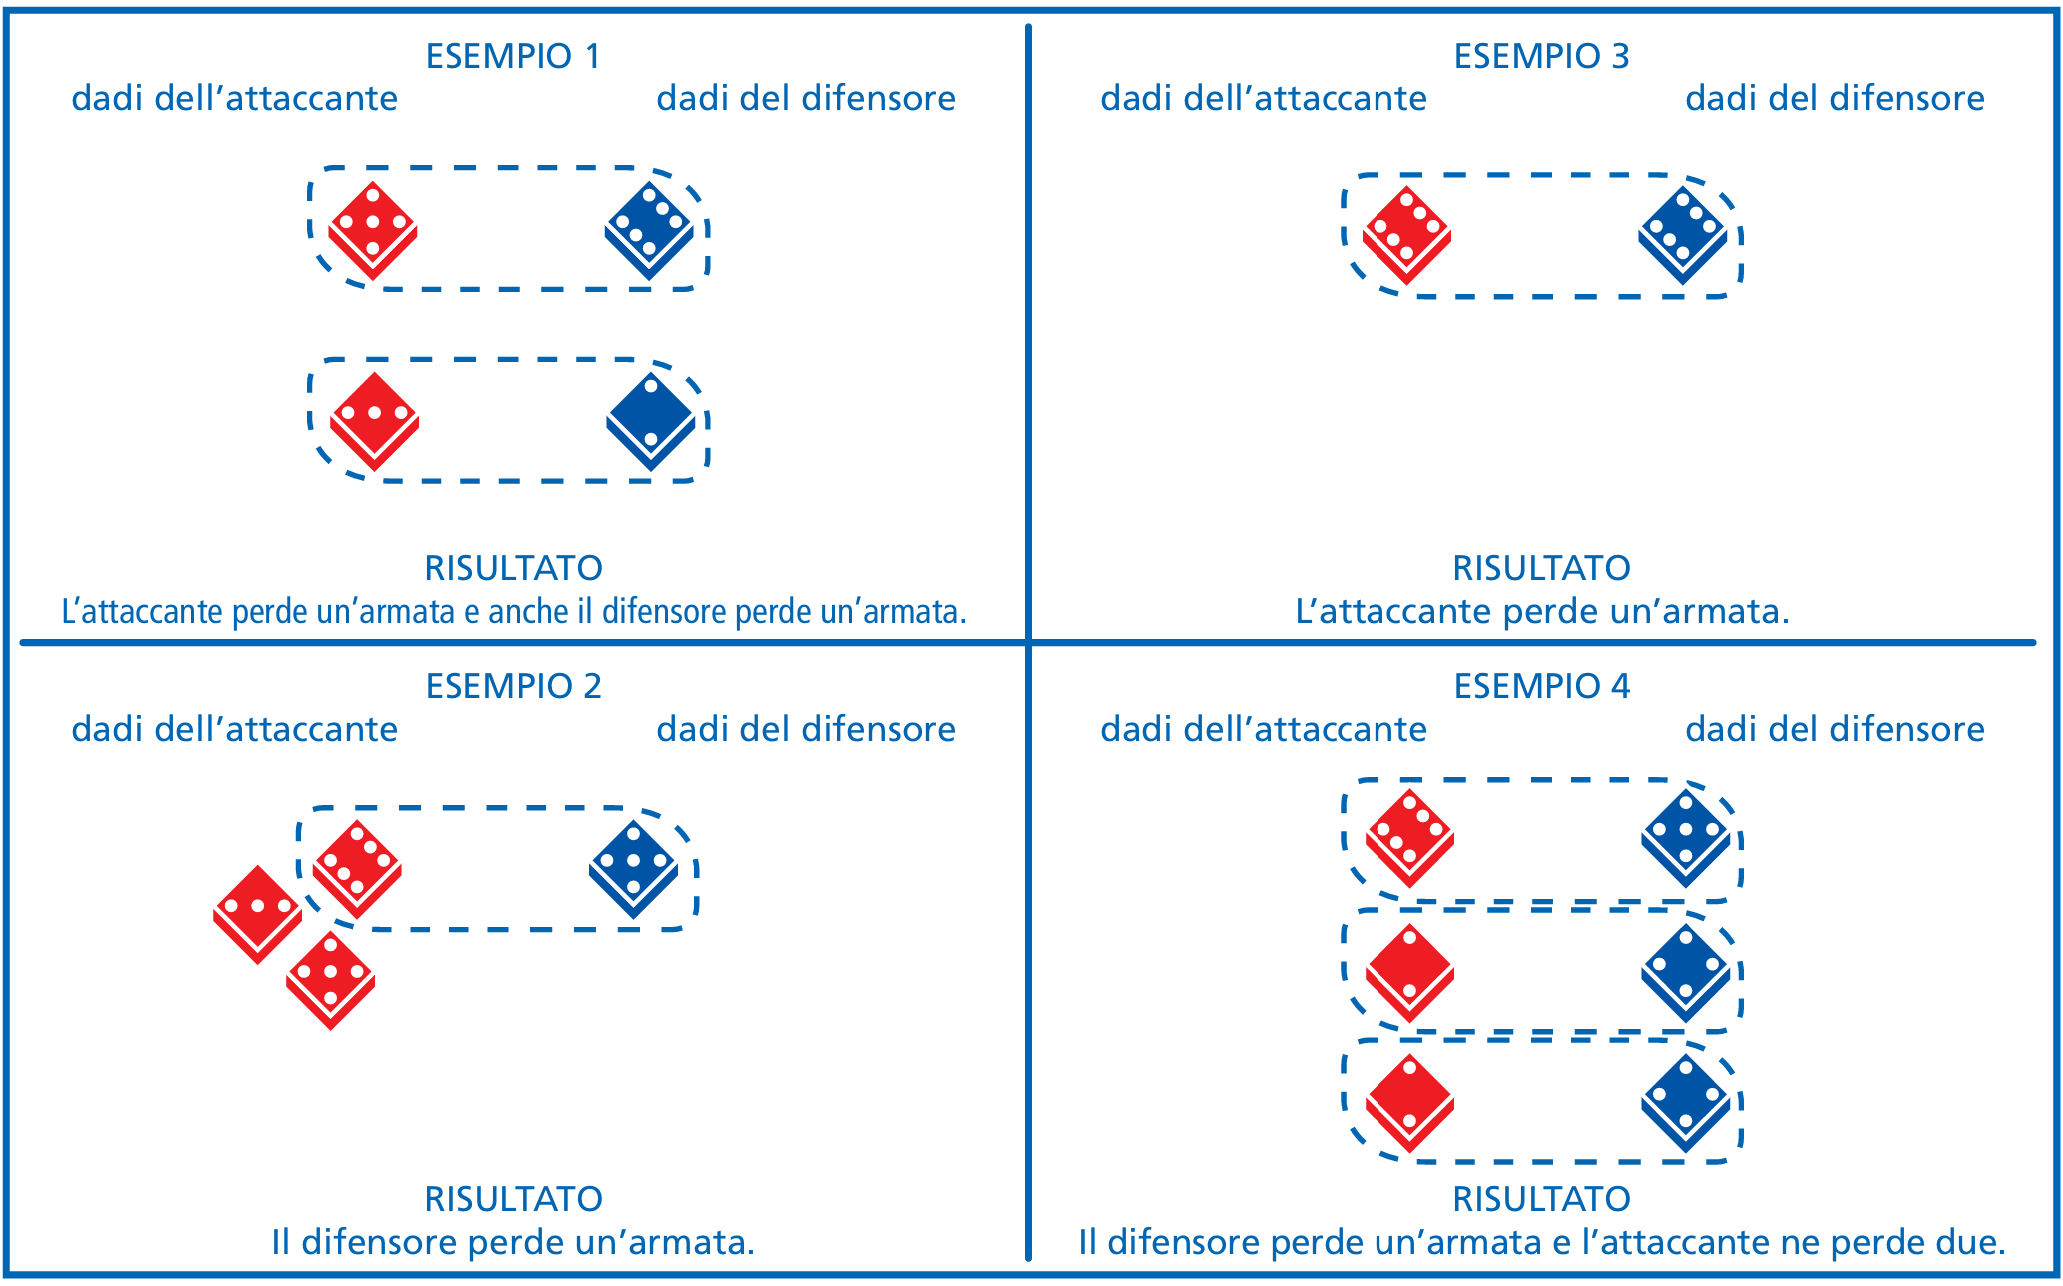
\includegraphics[width=1\textwidth]{user_guide/11_dice_rolls_examples.png}
	\caption{Esempi di tiri di dadi dal manuale di Risiko.}
\end{figure}

\section{Fase di spostamento strategico}
La fase di spostamento strategico permette di spostare delle unità da un territorio a un altro territorio adiacente, entrambi di proprietà del giocatore, corrente in un solo senso.

\begin{figure}[H]
	\centering
	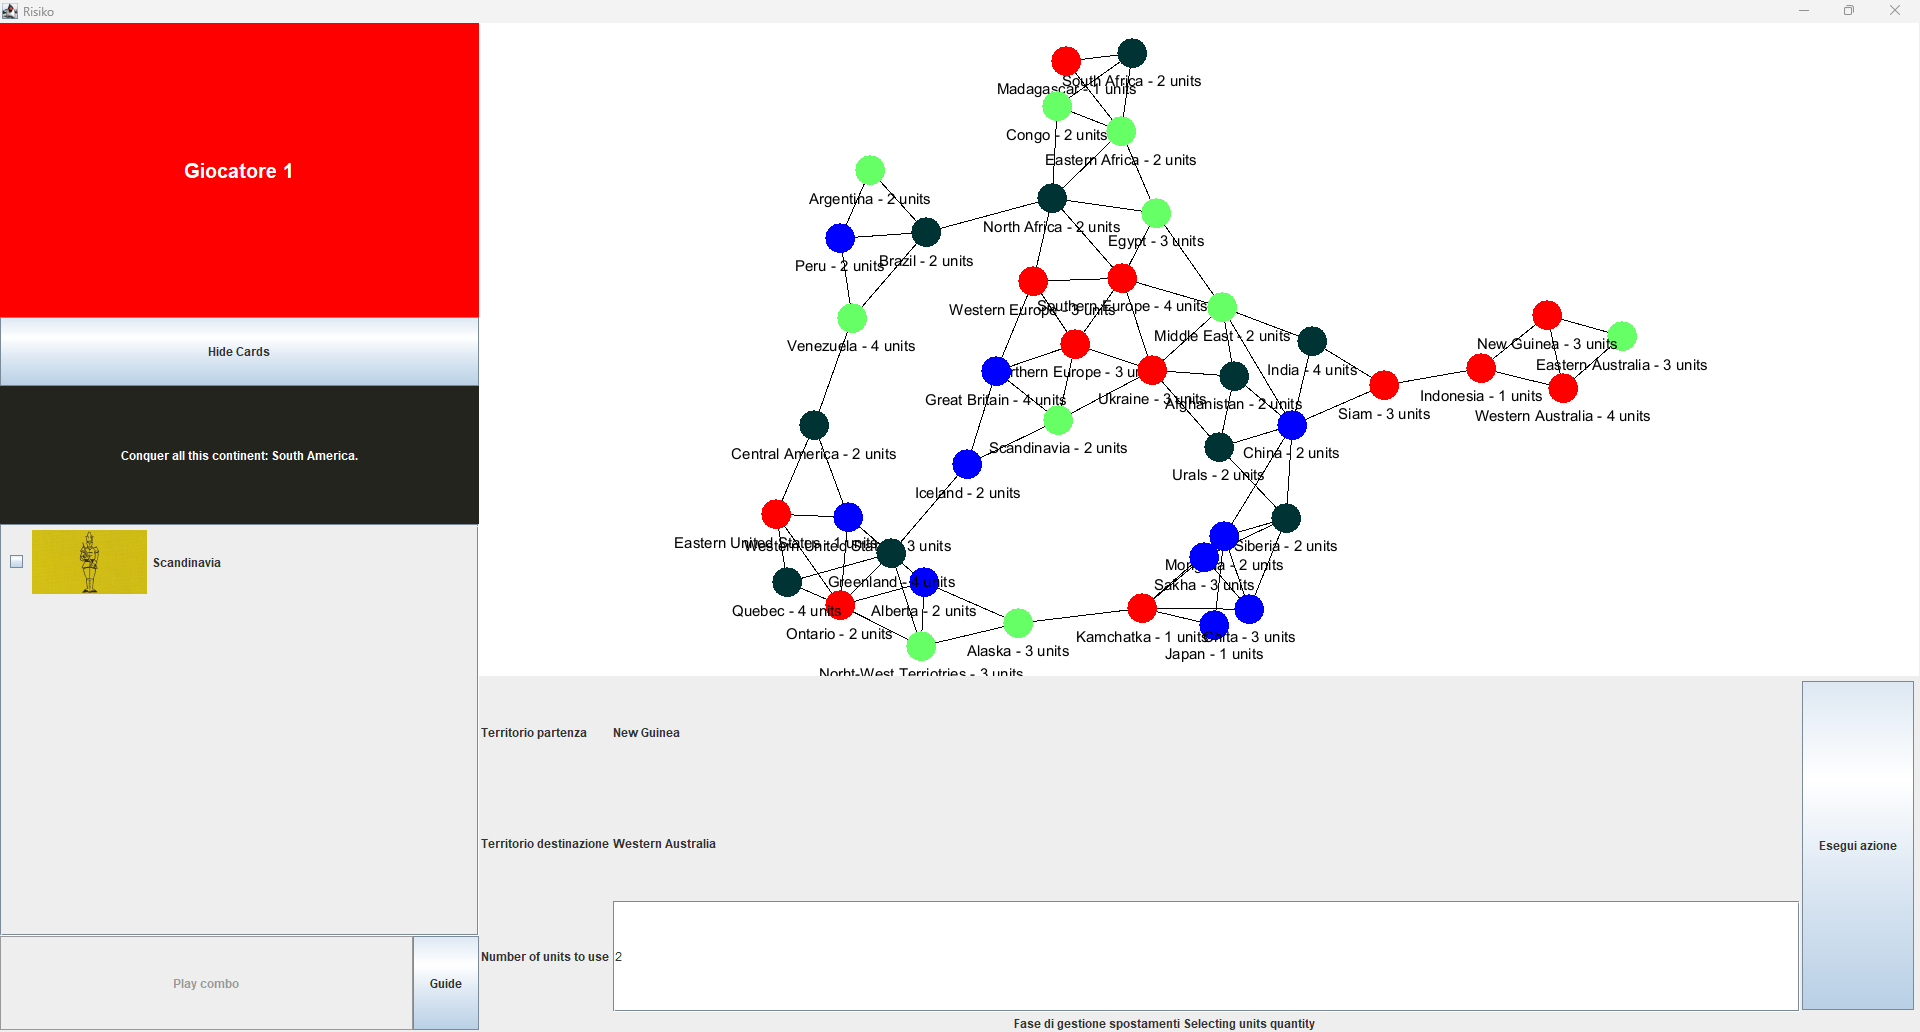
\includegraphics[width=1\textwidth]{user_guide/12_final_move_before.png}
	\caption{Spostamento di un'unità dalla Nuova Guinea all'Australia Occidentale.}
\end{figure}

Come nella fase di attacco, bisogna pianificare lo spostamento in vari passaggi, dopo ognuno bisogna cliccare il pulsante \textbf{Esegui azione} per passare al passaggio successivo:
\begin{enumerate}
	\item Cliccare il territorio da cui spostare le unità, facendo attenzione che abbia almeno due unità e che sia adiacente a un territorio dello stesso giocatore.
	\item Cliccare il territorio dove le unità verranno spostate. Dev'essere adiacente al territorio da cui si sta spostando e di proprietà del giocatore.
	\item Scegliere quante unità spostare, dev'essere un numero compreso tra uno e il numero massimo di unità in quello di partenza meno uno.
\end{enumerate}

Per confermare lo spostamento, cliccare sul pulsante \textbf{Esegui azione}.
Il turno del giocatore attuale è concluso, tocca quindi al giocatore successivo.

\section{Vittoria}
Un giocatore vince se riesce a completare il suo obiettivo.

\chapter{Esercitazioni di laboratorio}

\section{matteo.caruso7@studio.unibo.it}

\begin{itemize}
	\item Laboratorio 08: \url{https://virtuale.unibo.it/mod/forum/discuss.php?d=178723#p247198}
	\item Laboratorio 09: \url{https://virtuale.unibo.it/mod/forum/discuss.php?d=179154#p247764}
	\item Laboratorio 10: \url{https://virtuale.unibo.it/mod/forum/discuss.php?d=180101#p248784}
	\item Laboratorio 11: \url{https://virtuale.unibo.it/mod/forum/discuss.php?d=181206#p250854}
\end{itemize}

\section{matteo.ceccarelli@studio.unibo.it}
% TODO: Compila i laboratori che hai fatto e metti l'email giusta.
\begin{itemize}
	\item Laboratorio XX: \url{https://virtuale.unibo.it}
\end{itemize}

\section{franceso.sacripante@studio.unibo.it}
% TODO: Compila i laboratori che hai fatto e metti l'email giusta.
\begin{itemize}
	\item Laboratorio XX: \url{https://virtuale.unibo.it}
\end{itemize}


\bibliographystyle{alpha}
\bibliography{blbliography}
\end{document}